\chapter{Architecture}
This chapter discusses the changes made to the internal architecture of the application. While most of those changes were motivated by some technical need or issue, we also made changes so that it is possible to use a properly secured connection which helps us further protect the privacy of our users and the security of their data. The details about those change are explained in details in section \ref{sec:proxy} and in particular the subsection \ref{subsec:privacy} is aimed at explaining the implications and benefits on our users' privacy and security.
\section{Previous architecture}
The previous architecture has at its core goal to isolate as much as possible the processes handling our users' private data from the outside world. As can be seen in figure \ref{fig:fetchArch} and figure \ref{fig:gameCreationArch} the Game Creator (also sometimes called Game Generator) process does not accept request from the outside world and everything goes through the reminisceme component. This component itself accepts requests from the outside world but never handles the data we get from Facebook, it can only get the created game boards from the Game Creator, never the actual piece of data used to generate it.\\
While this architectures is really good at preventing private data from leaking to a potential malicious user (thanks to the fact that we authentify our user through Facebook authentification), it does not help the user to verify the identity of the server. This setup is quite vulnerable to what is called a Man-in-the-middle attack\cite{mitm} and the communication is not encrypted. In short, a malicious person could (with more or less ease) intercept messages and read the generated questions (which contain some of the user's Facebook data). A simple solution to this is the use of SSL\cite{whyssl}\cite{ssl} certificates. Those certificates enable trust (it gives a way for the user's browser to check our identity through a Certificate Authority\cite{ca}, we used Let's Encrypt\cite{letsencrypt} because it is free, easy to use and trusted.).
\begin{figure}[!h]
\center
{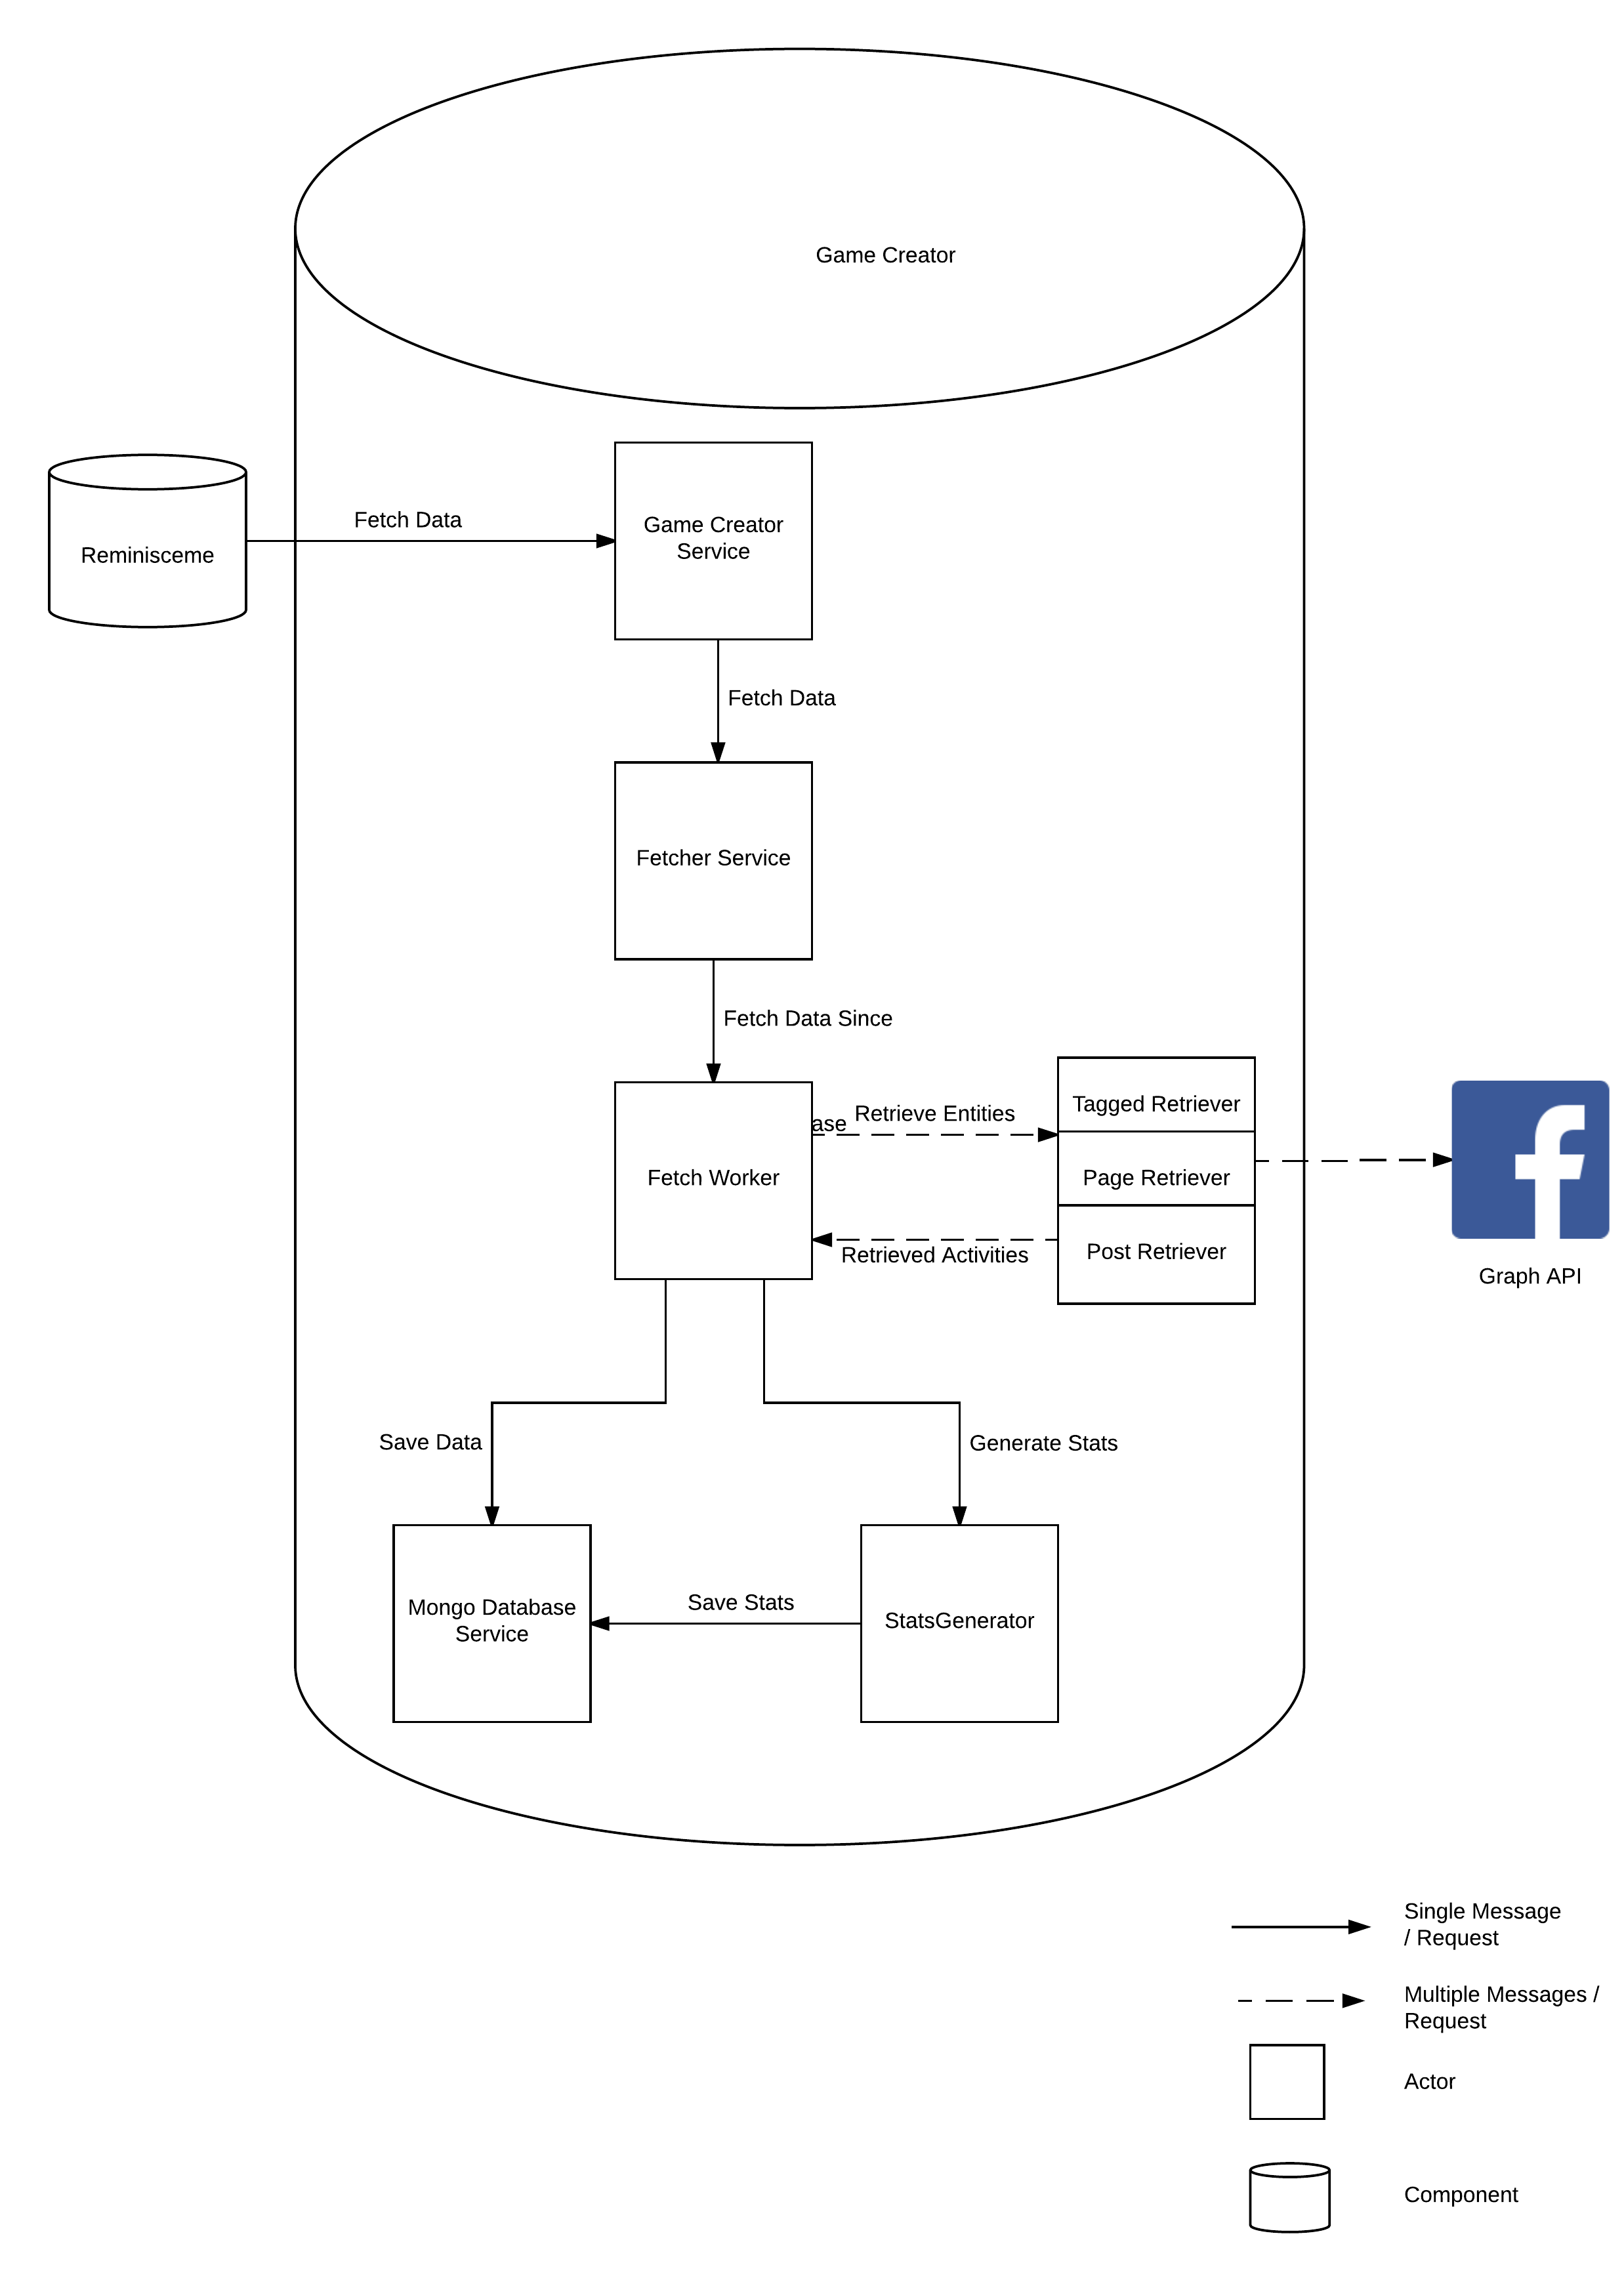
\includegraphics[width=3.5in]{images/fetch_arch.png}}
\caption{Fetching architecture schema}
\label{fig:fetchArch}
\end{figure}
\begin{figure}[!h]
\center
{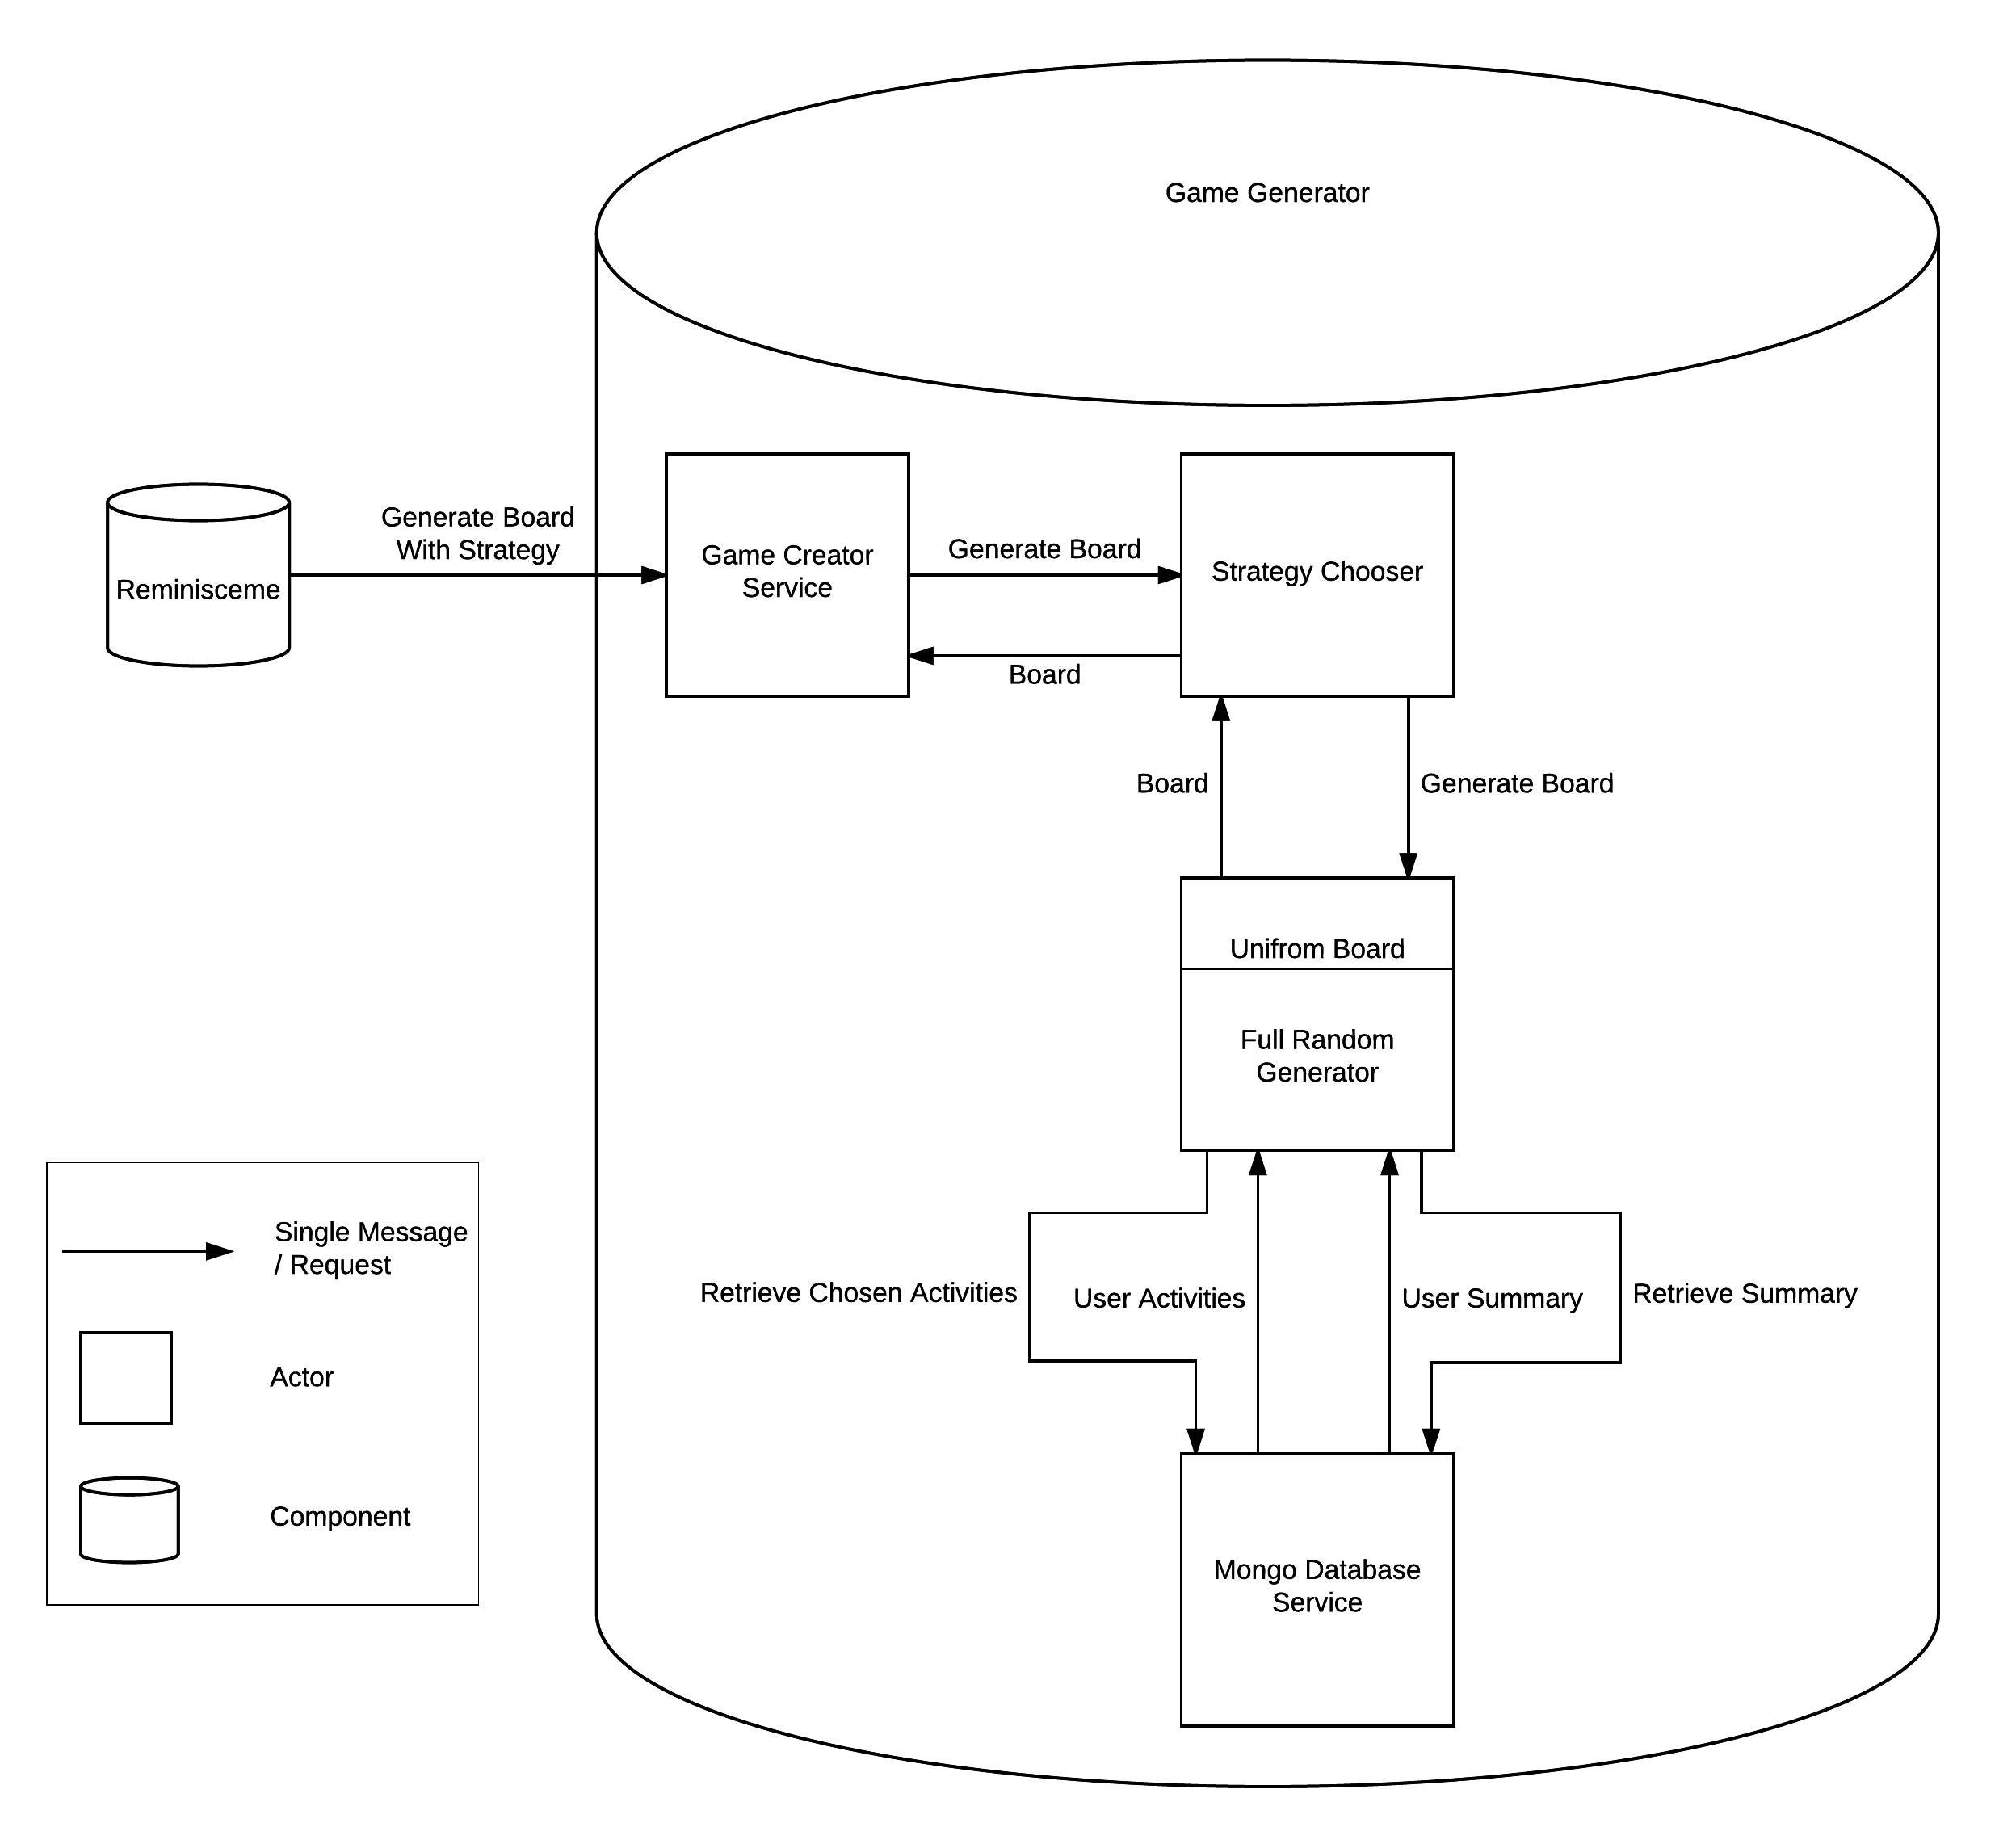
\includegraphics[width=3.5in]{images/gc_arch.png}}
\caption{Game generation schema}
\label{fig:gameCreationArch}
\end{figure}
\section{A proxy to face the world}\label{sec:proxy}
Using SSL certificates properly implies doing a lot of sometimes complicated cryptographic work. It is never advised try and implement this kind of protocol by oneself. In fact it is one of the most common security mistake. This is the first reason we needed to introduce a proxy\cite{reverseproxy}. It is a piece of software that will serve as a single point of communication between the "outside world" and our application. Most of the modern proxies are simply able to use the SSL protocol and serve the requests to our application in a transparent way. Which means that, by simply adding a proxy in font of our application we can add a lot of privacy protection and trust (more in subsection \ref{subsec:privacy}).\\
A second reason we were interested in having a proxy in place is that we wanted to have some administrative tools available easily from the same server as the application (in particular we wanted to be able to easily consult the logs (\ref{sec:logging}) generated by the application if anything went wrong) and a proxy's main function is actually to serve information from multiple processes on a single access point.\\
Finally it can also be seen as "doubling" the isolation of the Game Creator by putting an other layer of protection on top of the previous one, while not necessarily mandatory, it is always a good idea to rely on tested and widespread software rather than our own only when it comes to security.\\
We decided to use NginX\cite{nginx} for the above-mentioned reasons, a lot of people use it (which also means that it is easier to find information about it online), it has been proven reliable and powerful and it supports a lot of useful features such as preventing user to access the server without using the SSL protocol (everything is handled in a transparent way and the user never has to think about it).
\subsection{Privacy and security}\label{subsec:privacy}
To understand the benefits of using a proper SSL certificate and protocol, it is important to understand a bit more about how it works. As mentioned before, it is used mainly to allow the user to identify the server or website as being who it is pretending to be and to allow encryption of the exchanged messages. Any well-configured server using SSL will be able to show a certificate to the user's browser which the latter can verify with the Certificate Authority which produced it. The Certificate Authority will make sure that:
\begin{enumerate}
	\item The certificate is indeed the valid one for the visited website.
	\item The person which originally generated the certificate is the owner of the website which is being certified.
	\item The certificate has not been revoked by its owner
\end{enumerate}
If those conditions are met, the browser will be able to trust the website and the user will have a visual confirmation that this site can be trusted (it usually is a green lock or text in the address bar ads shown in figure \ref{fig:sslBar}). The browser can also now establish a securely encrypted connection with the server preventing anyone from reading the messages exchanged. When the user sees that the website is trusted by the browser, they can trust that their data is handled in a responsible way. As a side note, it is possible to assess the quality of the configuration of a server by using a testing benchmark, for instance, here are the results for the domain \url{reminisce.me} on the Qualys SSL Labs benchmark\cite{ssllabs}: \url{https://www.ssllabs.com/ssltest/analyze.html?d=reminisce.me}.
\begin{figure}
\centering
{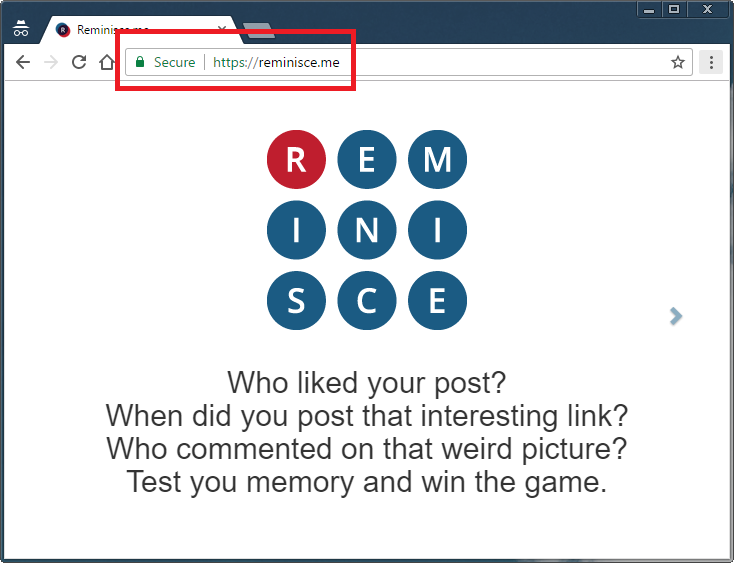
\includegraphics[width=3.5in]{images/ssl_bar.png}}
\caption{Trusted website}
\label{fig:sslBar}
\end{figure}
\section{Monitoring and logging}\label{sec:logging}
When developing and maintaining an application, one of the key feature required to be able to find, understand and eliminate defect, is the ability to understand the failure. One need to be able to see where the failure happened, what the state of the system was and if possible the cause of the failure. In order to achieve this, a well thought logging system is mandatory. This means that the application must produce logs that are readable and explanatory, they must provide as much information as possible so that the cause of failure can be identified rapidly. On top of this, one need to be able to search through the logs in a convenient way, which is not a given because with a large number of user the log can start to grow a lot.\\
One of the common usage of the log is to find why one user encountered the problem which was reported, when this is the case we need to be able to find all actions performed by the application for that user. With this in mind, we made sure that whenever possible an identifier for the user who triggered the action is added to the log.
\subsection{Indexing the log and looking at it}
We wanted to be able to easily answer questions such as "How often does this problem happen?". To be able to do this in the easiest way, we have to provide a search interface which provides tools for searching and analyzing the logs. Fortunately, this is a common issue when building an application so solutions already exist. We decided to use ElasticSearch\cite{elasticsearch} and Logstash\cite{logstash} to index the logs. As shown on figure \ref{fig:loggingArch}, the Game Creator and the application both write their logs to a file, Logstash then reads those files and feeds them into the ElasticSearch database which then makes them easily searchable (by using the Elastic Search Query DSL \cite{querydsl}). Finally we use Kibana\cite{kibana} to have a nice graphical interface to access the indexed logs. It provides ways to formulate queries and generate graphs which can help monitor certain events such as the number of detected failures. Figure \ref{fig:kibana} shows an example of the graphical interface Kibana provides. It is worth noting that access to this graphical interface is protected by an authentication scheme based on session cookies (SEE APPENDIX).%TODO: APPENDIX ON COOKIES FOR LOGS
\begin{figure}
\centering
{\includegraphics[width=3.5in]{images/logging_arch.png}}
\caption{Logging architecture}
\label{fig:loggingArch}
\end{figure}
\section{Stats module}
\begin{figure}
\centering
{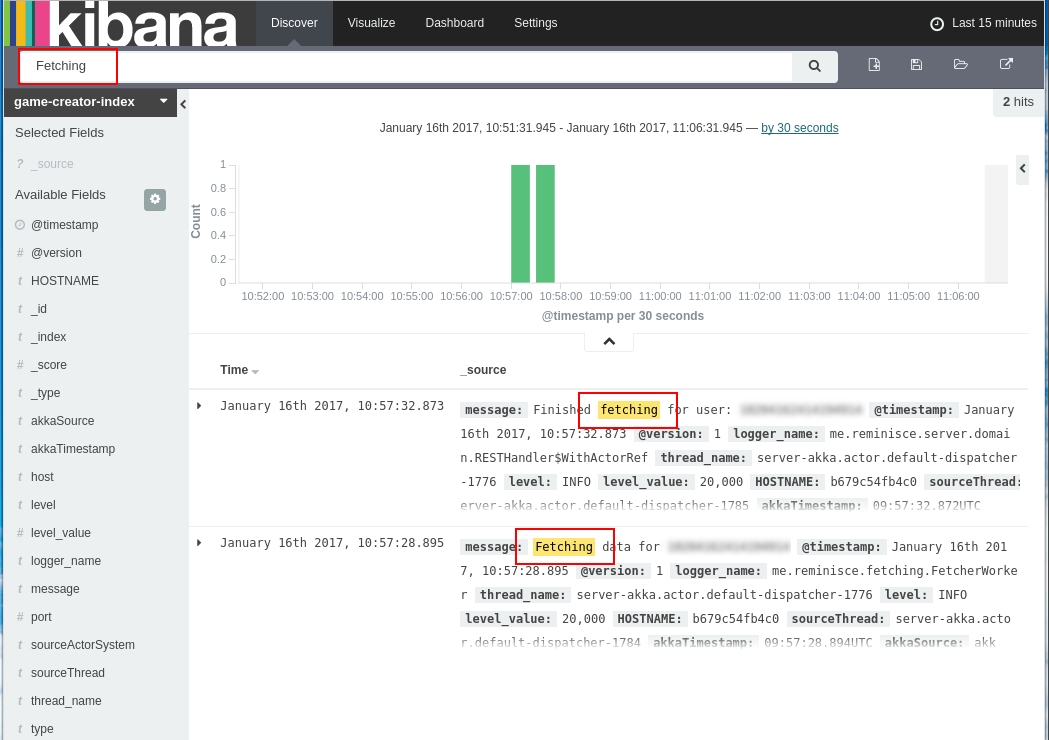
\includegraphics[width=6in]{images/kibana.png}}
\caption{Kibana Logs Interface}
\label{fig:kibana}
\end{figure}
\section{Stats module}

1. Simplification to make it easier to use and extend
2. Added time spent
3. Display to the user to make it more enjoyable.